\section{Results}

The analysis considered two levels. The first level comprises general observations regarding interaction with
the AI system, which were derived from the transcripts and recordings of the user studies. This level
describes overarching observations and was linked to the user studies. The second level consists of the
analysis of the participants’ perceptions regarding the meeting in general as well as the AI facilitator.
This is based on the questionnaire, which specifically includes open-ended responses.
% ---------------------------------------------------------------------------------------------------------------------
\subsection{General Observations and link to user stories}

Overall, five of the six user stories were addressed by the system during its interactions. The only
exception was User Story 1, which concerned addressing the meeting agenda or goal. The system did not refer
to either the agenda or the meeting objective in any of the three user studies. However, the system remained
neutral throughout all three studies and did not make decisions on its own, thereby fulfilling User Story 6.

Regarding User Story 5, which aimed to ensure that the system intervened sparingly and only when doing so
clearly added value, the overall impression was that the system intervened too frequently.

\begin{table}[H]
  \centering
  \caption{Frequency of spoken AI interventions in the three user studies.}
  \label{tab:intervention-frequency}
  \footnotesize
  \begin{tabular}{@{}lrrr@{}}
    \toprule
    Group & AI contributions & Session length (min) & Interventions per minute \\
    \midrule
    G01 & 19 & 20 & 0.95 \\
    G02 & 12 & 25 & 0.48 \\
    G03 & 11 & 19 & 0.58 \\
    \bottomrule
  \end{tabular}
\end{table}

For the remaining user stories, specific interactions could be clearly identified and assigned to the
respective user stories. The following table presents the number of system interactions that could be
unambiguously attributed to each user story, along with examples of how these interactions were phrased.

\begin{table}[H]
  \centering
  \caption{System interactions attributed to user stories, with one example AI-Facilitator utterance each.}
  \label{tab:user-story-interactions}
  \footnotesize
  \begin{tabularx}{\textwidth}{@{}
      >{\RaggedRight\arraybackslash}p{3.6cm}
      ccc
      >{\RaggedRight\arraybackslash}X
    @{}}
    \toprule
    User story & G01 & G02 & G03 & Example \\
    \midrule
    \usref{us:quiet-voices}\newline
    {\scriptsize Balanced participation}
    & 3 & 2 & 3
    & \enquote{Then I'd like to briefly bring L.\ and M.\ into the discussion.
    What criteria are important to you when making this decision?}
    \textit{\scriptsize(G03)} \\
    \addlinespace[0.45em]
    \usref{us:unshared-information}\newline
    {\scriptsize Ensuring information completeness}
    & 4 & 5 & 3
    & \enquote{D., is there anything else about Stevens, Roberts, or Jones that's
    important for the comparison and hasn't been mentioned yet?}
    \textit{\scriptsize(G02)} \\
    \addlinespace[0.45em]
    \usref{us:hold-dissent}\newline
    {\scriptsize Preserving dissent}
    & 2 & 2 & 3
    & \enquote{My takeaway is that we should make sure to consider the opposing
    viewpoints on all three candidates before we rule anyone out too soon.}
    \textit{\scriptsize(G02)} \\
    \bottomrule
  \end{tabularx}
\end{table}

In addition to the interactions listed above, some system interactions could not be clearly assigned to a
single user story, while others addressed two user stories simultaneously. In particular, the system
frequently combined User Stories 2 and 3 in its interventions.

Furthermore, several additional issues with the AI agent's behavior were observed, affecting both the
naturalness of the interaction and the system's acceptance. In some cases, the agent did not complete an
ongoing thought but interrupted its own utterance to express a newly emerging thought instead.
{\setlength{\topsep}{0.25\baselineskip}\setlength{\partopsep}{0pt}%
  \begin{quote}\small
    \enquote{Thank you, F. I hear the point about engagement and the possible interpretation\ldots}\\
    \enquote{Thank you, J. The point is important when we consider Jones' positi—\ldots}\\
    \enquote{Thank you, F. You are already close to the key distinctions. To ensure that we
      move beyond impressions, what would be the clearest exclusion criterion for Jones, if
    there is one?}
\end{quote}}

Although this behavior theoretically allowed the agent to incorporate new information into the interaction as
it emerged, it unnatural. The existing system design lacked a mechanism for naturally
integrating a newly emerging thought into an utterance that had already begun. This limitation highlights a
gap in the system design.

Another recurring observation was the increasing tendency of participants across all three groups to ignore
the AI agent's interventions, either occasionally or over extended periods. This behavior manifested in
participants not responding to the agent's contributions or continuing their conversations while the agent
was speaking. A lack of contextual awareness and poorly timed interventions appeared to be contributing
factors. Some differences were observed between the groups. In Group 2, a participant suggested ignoring the
AI agent after only its second interaction. Group 1 also gradually developed a tendency to largely disregard
the agent's interventions and continue their own conversation without interruption while the agent was
speaking (8/19 Interactions). In Group 3, by contrast, participants initially appeared confused by the
agent's interaction behavior. They seemed to suspect a delay in the AI's processing of the conversation and,
particularly at the beginning, sometimes waited for its responses. This was especially apparent when the
agent asked a question: after answering, participants appeared to expect the AI to provide further input or
contextualize their responses. Participants sometimes responded immediately by verbally expressing their
frustration. This is illustrated by a statement made by a participant during User Study 3:
“I would, if you didn't keep interrupting me.”

Regarding the hidden-profile scenario, the following observations were made: Of the three groups, only Group
2 selected the ideal candidate. This group recognized on its own and early on that it was in a hidden-profile
scenario. Group 1 did not notice until toward the end of the meeting (around the 16-minute mark) that they
apparently had different information about the candidates. While the group was confused by the seemingly
inconsistent information, the AI facilitator suggested clarifying exactly which candidate should be assigned
each negative trait.

% ---------------------------------------------------------------------------------------------------------------------
\subsection{Perceived Meeting Quality (Davison Instrument)}

\paragraph{Comparison across groups}\mbox{}\\*[0.75ex]
\noindent
The median scores of the groups on the Likert-scale items were compared across the three user studies.
Differences of less than 1.5 scale points were considered insignificant.
No larger difference was found, except on four items:
\begin{itemize}
  \item D2 (appropriate--inappropriate), with medians of 4.5 (G01),  3 (in G02) and 5 (in G03);
  \item T2 (the members worked together as a team), with medians of 5 (G01), 4.5 (G02) and 3 (G03);
  \item E2 (meeting time was used efficiently), with medians of 5 (G01), 4.5 (G02) and 2.5 (G03)
  \item A4a (AI intervened too rarely.), with medians of 5 (G01), 4.5 (G02) and 3 (G03);
\end{itemize}
These discrepancies do not show that one group differed from the others across the entire Davison instrument.
On every other Likert item the three group medians stayed within 1.5 scale points, and the lower median is
not the same group in each case: G02 on D2, and G03 on T2, E2, and A4a.
The four gaps therefore concern different groups and point in different directions, which is why the ratings
are still plotted together.

\paragraph{Communication}\mbox{}\\*[0.75ex]
\noindent
\begin{minipage}{\linewidth}
  \centering
  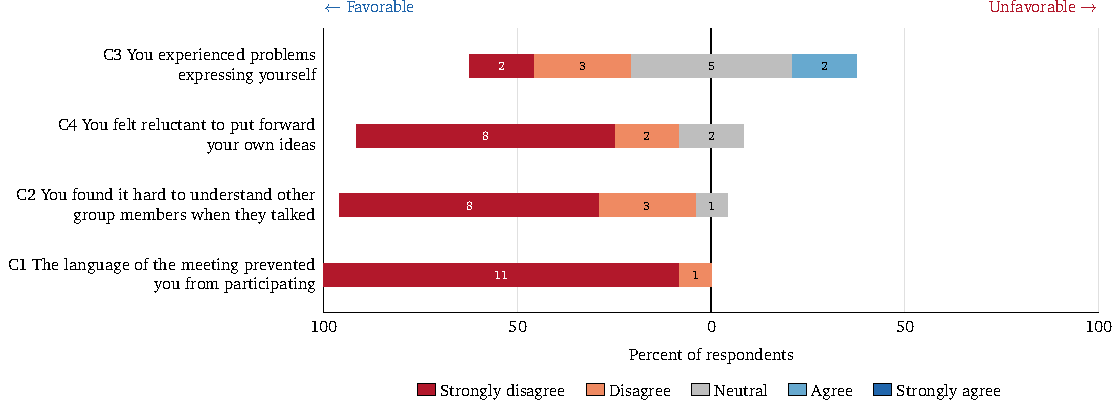
\includegraphics[width=\linewidth]{assets/figures/05/likert-communication.pdf}
  \captionof{figure}{Perceived communication (Davison items C1--C4). Each bar shows the share of responses on the
    five-point scale.
  \figsource{Own illustration.}}
  \label{fig:likert-communication}
\end{minipage}

The perception of the ability to express one's opinion is the most negative. This may be attributable to the
high interaction rate of the AI and the resulting interruptions.

\paragraph{Quality of discussions}\mbox{}\\*[0.75ex]
\noindent
\begin{minipage}{\linewidth}
  \centering
  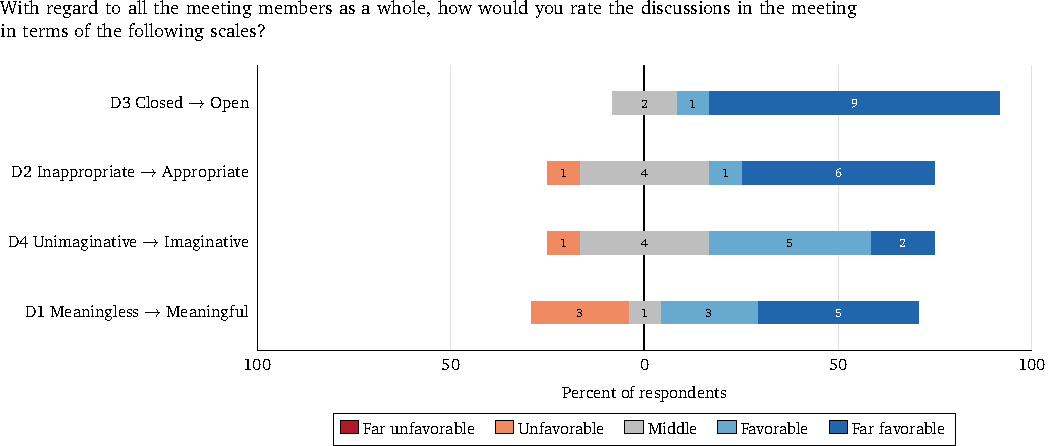
\includegraphics[width=\linewidth]{assets/figures/05/likert-discussion.pdf}
  \captionof{figure}{Perceived discussion quality (Davison items D1--D4). Each bar shows the share of
    responses on the five-point semantic differential. The marker above the scale names the
    unfavorable and favorable ends. Counts are illustrative.
  \figsource{Own illustration.}}
  \label{fig:likert-discussion}
\end{minipage}

The quality of the discussion is viewed positively

\paragraph{Status effects}\mbox{}\\*[0.75ex]
\noindent
\begin{minipage}{\linewidth}
  \centering
  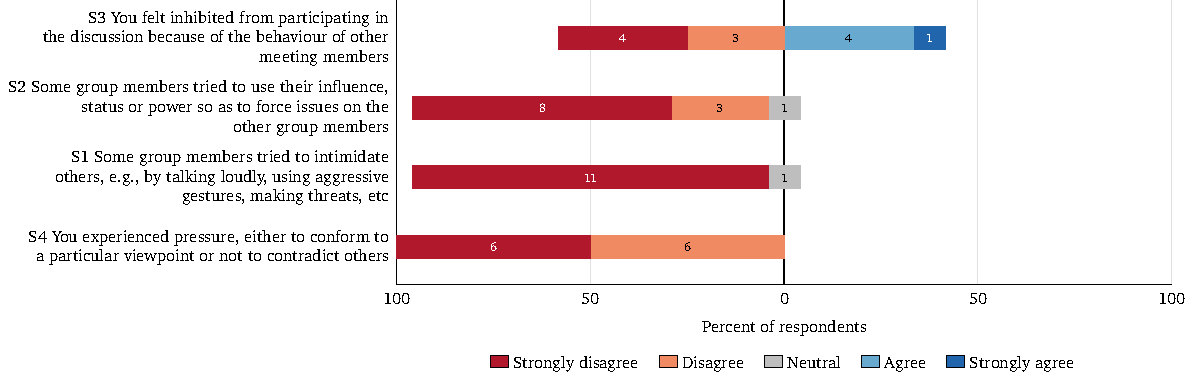
\includegraphics[width=\linewidth]{assets/figures/05/likert-status.pdf}
  \captionof{figure}{Perceived status effects (Davison items S1--S4). Each bar shows the share of responses on the
    five-point scale.
  \figsource{Own illustration.}}
  \label{fig:likert-status}
\end{minipage}

There do not appear to have been any disruptive factors affecting the status effects. Only S3 shows negative
tendencies. This could be due to the fact that the participants classified the AI as a meeting participant,
and the negative tendencies therefore relate to the AI facilitator.

\paragraph{Team work}\mbox{}\\*[0.75ex]
\noindent
\begin{minipage}{\linewidth}
  \centering
  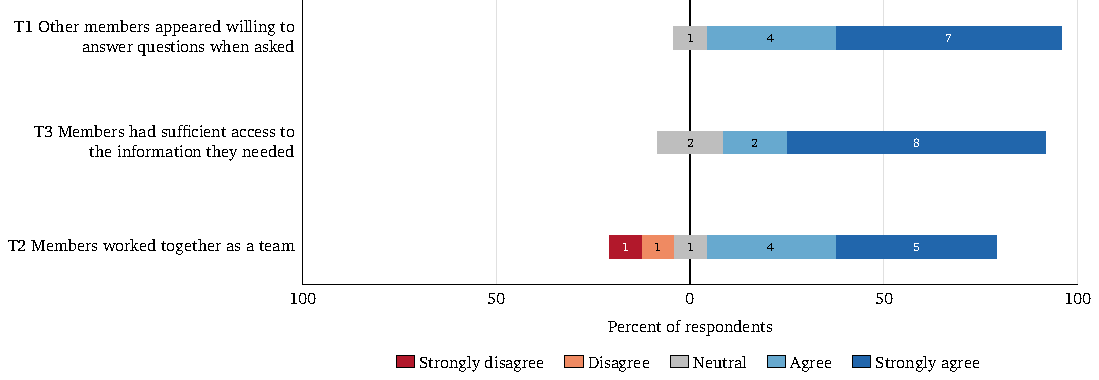
\includegraphics[width=\linewidth]{assets/figures/05/likert-teamwork.pdf}
  \captionof{figure}{Perceived teamwork (Davison items T1--T3). Each bar shows the share of responses on the
    five-point scale.
  \figsource{Own illustration.}}
  \label{fig:likert-teamwork}
\end{minipage}

There were no predominantly negative trends in teamwork either, with the exception of T2. Similar to S3, this
can also be attributed to the wording of the question, which theoretically allows the AI facilitator to be
considered part of the team.

\paragraph{Efficiency}\mbox{}\\*[0.75ex]
\noindent
\begin{minipage}{\linewidth}
  \centering
  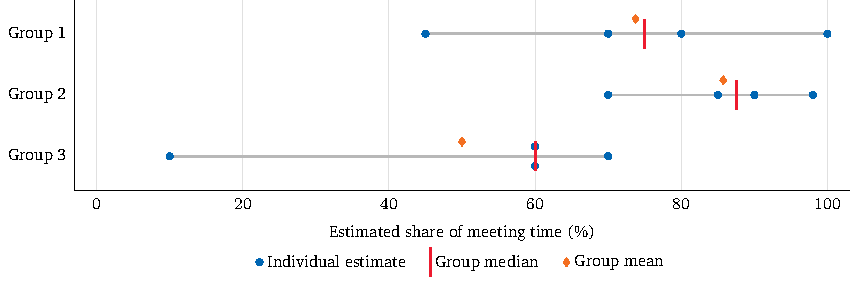
\includegraphics[width=\linewidth]{assets/figures/05/efficiency-share.pdf}
  \captionof{figure}{Estimated share of meeting time spent in serious discussion (Davison item E4).
    Each dot is one participant. The line spans the lowest and highest estimate in that group.
    The vertical mark is the group median, and the diamond is the group mean.
  \figsource{Own illustration.}}
  \label{fig:efficiency-share}
\end{minipage}

The median perceived efficiency ranged from 60\% to 85\%. However, no direct correlation was found between
efficiency and the AI facilitator's interactions.

% ---------------------------------------------------------------------------------------------------------------------
\subsection{Participants' Perception of the Proactive AI Moderator's Interventions}
\label{sec:participant-perception}

This section explicitly describes how the AI facilitator was perceived by the participants.
\paragraph{Disruption and frequency}\mbox{}\\*[0.75ex]
\noindent
\begin{minipage}{\linewidth}
  \centering
  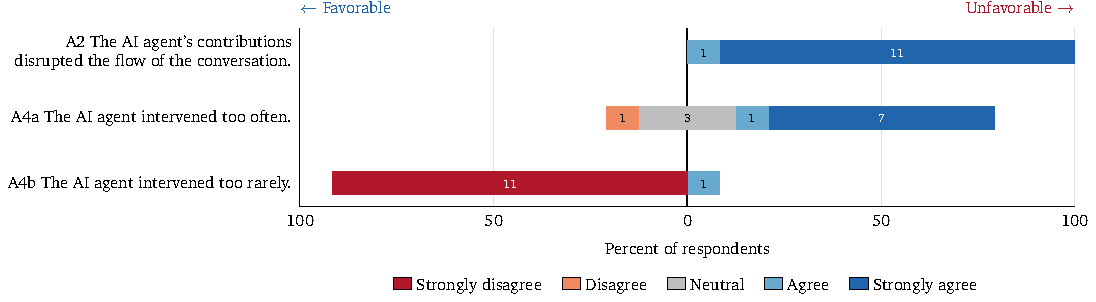
\includegraphics[width=\linewidth]{assets/figures/05/likert-agent-2.pdf}
  \captionof{figure}{Perceived disruption and intervention frequency of the proactive AI agent
    (items A2, A4a, and A4b). Each bar shows the share of responses on the five-point scale.
    Counts are illustrative.
  \figsource{Own illustration.}}
  \label{fig:likert-agent-2}
\end{minipage}

Es bestand eine ganz klare zustimmung das die Beiträge des KI-Facilitator die diskussion gestört haben.
zusätzlich bestand einigkeit darüber dass die KI zu oft interagiert hat.

G1-P2 beschreibt dies wie folgt: "Sie ist nach jedem Redebeitrag angesprungen und hat den Redefluss dann sehr
stark eingeschränkt."

Nru eine Person gab an die KI habe zu selten intervieniert.
G1-P4 beschreibt eine möglich erklärung dafür wie folgt: "Also zusammengefasst kam es mir so vor, als ob die
ki viel zu oft an unpassenden Stellen störend eingegriffen hat und dafür an anderen Stellen, weniger, wo es vielleicht
jemand gebraucht hättet, der jetzt die Leere füllt. "

\paragraph{Agent attributes}\mbox{}\\*[0.75ex]
\noindent
\begin{minipage}{\linewidth}
  \centering
  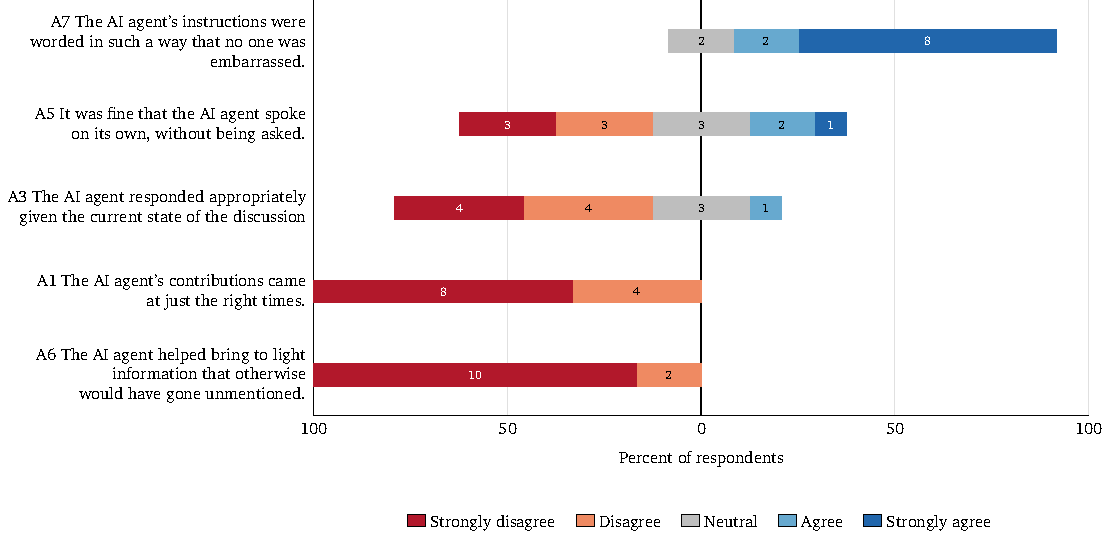
\includegraphics[width=\linewidth]{assets/figures/05/likert-agent-1.pdf}
  \captionof{figure}{Perceived attributes of the proactive AI agent (items A1, A3, A6, A7, and A8).
    Each bar shows the share of responses on the five-point scale. Counts are illustrative.
  \figsource{Own illustration.}}
  \label{fig:likert-agent}
\end{minipage}

Zu A7 äußerten sich 8 Teilnehmende positiv und lediglich zwei neutral. Bei den Teilnehmden hersschte eine
klar tendenz dazu dass es gut war das war wie der KI-Faciliator agiert.
G3-P4: "An sich ist es positiv, dass explizit auch Leute angesprochen werden, dadurch konnten generelel auch
Leute zur Sprache kommen, die sich sonst eher zurückhalten."
G3-P2 mwekr an, dass er es gut fand , dass die KI anerkennend war. G1-P1 erkannte ein wieder kehrendes Muster
bei den Beiträgen der KI:
{\setlength{\topsep}{0.25\baselineskip}\setlength{\partopsep}{0pt}%
  \begin{quote}\small
    \enquote{Die KI hat sich dann immer bedankt, das zuletzt Gesagte zusammengefasst
    und ihre Frage formuliert.}~\textit{\scriptsize[G1-P1]}
\end{quote}} Auch G1-P2 beschreiben diese Muster aber als leicht nervig auf grund der hohen wiederholung.

A3 legt nahe dass die anworte der KI unpassend zum akteullen kontext waren. dies ist verbunden mit dem
Zeitpunkt der interaktion A1 ,welche als noch negativer wahrgenommen wrude. Eine korrekte Interatkion die
eigentlich sinnvoll gewesen wäre nun zu spät kommt wird als störend wahrgenommen so sagt G3-P1: "Inhallich
waren die Beiträge gut, allerdings verzögert, oder hinter unserem Denkprozess"
G1-P4 sagt dass er sich hauptsächlich an situation erinnert indenen die KI zum falschen Zeitpunkt eingegiriffen hat.
G3-P4 beschreibt es wie folgt:
{\setlength{\topsep}{0.25\baselineskip}\setlength{\partopsep}{0pt}%
  \begin{quote}\small
    \enquote{Die KI hat verzögert reagiert, dadurch Gespräche unterbrochen, ohne
    einen Mehrwert zu liefern.}~\textit{\scriptsize[G3-P4]}
\end{quote}}
Wurden teilnehmde druch die KI unterborchen empfenden diese das als störend, insbesondere wenn der
beitrag dann nicht zum kontext gepasst hat. so saget G2-P1 "Die KI hat mich beim Spreechen unterborchen udn
wollte auf ein anderes Thema lenken, was aber nicht im Konsenz mit dem momentaten Gruppenziel war, also im
Prinzip wars störend"
diese verzögerung wrude von eingen kandiaten beobachtet.
G3-P3 erkannte zwar an weshalb er unterbochen wurde auch wenn es ihn gestört hat: "In meinen Augen war hilfreich
das sie mich unterbrochen hat um {Name von G3-P1} und {Name von G3-P4} mehr raum zu geben, das war gut, auch
wenn es mich gestört hat "
Außerdem gab es Interaktione in dnen die KI den kontext falsch verstande hat und eine falsch aussage geätitgt
hat. G1-P2 beschreibt eine situation in der die KI dem falschen Kandiaten eine negative Eigenschaft zu geschreiben hat.
Andere Teilnehmende, wie zum Beispiel G1-P4, konkretisieren, dass die KI Personen
verwechselt hat:
{\setlength{\topsep}{0.25\baselineskip}\setlength{\partopsep}{0pt}%
  \begin{quote}\small
    \enquote{Gestört hat auch, dass sie die Person verwechselt hat.}~\textit{\scriptsize[G1-P4]}
\end{quote}}

Bei A6 scheinen die Befragen sich einige zu sein, dass der KI-Facilitator nicht dabei geholfen hat infromationen zu
enthüllen die sonst unerkannt blieben. Gleichzeitg beschreiben einige Kandidaten aber eingeschaften, die auf
gegentieliges hindeuten. so sagt G1-P2: "{Name von G1-P4} ist eher stiller bei der Diskussion gewesen und
wurde durch die KI gezielt angesprochen, sodass auch seine Meinung in Ruhe angehört werden konnte." weiter
beschreibt G1-P4:
{\setlength{\topsep}{0.25\baselineskip}\setlength{\partopsep}{0pt}%
  \begin{quote}\small
    \enquote{Die Situation, wo die KI aufgelöst hat, dass wir unterschiedliche
    Informationen hatten, war wahrscheinlich das Hilfreichste.}~\textit{\scriptsize[G1-P4]}
\end{quote}}
{\setlength{\topsep}{0.25\baselineskip}\setlength{\partopsep}{0pt}%
  \begin{quote}\small
    \enquote{Die KI hat explizit Teilnehmer angesprochen und nach deren Meinung zu
      etwas Speziellem gefragt. Das fand ich hilfreich, um alle Perspektiven zu
    erhalten.}~\textit{\scriptsize[G1-P1]}
\end{quote}}

Abschließend ist in diesem Kontext die  A5 liegen überraschende Ergebnisse vor.
Obwohl die Störung als hoch wahrgenommen wurde und auch die Interventionsfrequenz
deutlich zu hoch war, gaben lediglich 6 der 12 Teilnehmenden an, nicht zuzustimmen,
dass es in Ordnung war, dass der KI-Agent von allein gesprochen hat.
Die anderen 6 hatten eine neutrale Ansicht oder stimmten sogar zu, dass es in
Ordnung war, dass die KI aktiv gesprochen hat.

%_____

Weiter negativ aufgefallen ist die Lönge der Interaktion und das komplette ausreden.
G1-P1"Wenn sie unterbrochen hat, hat sie immer komplett ausgeredet, auch wenn der Einwand unnötig war"

Bei A3 stimmen die Teilnehmenden nicht zu, dass der KI-Agent für den Kontext
angemessen reagiert hat.
So beschreibt beispielsweise G2-P2:
{\setlength{\topsep}{0.25\baselineskip}\setlength{\partopsep}{0pt}%
  \begin{quote}\small
    \enquote{Leider sehr störend, da die KI nicht wirklich den Kontext verstanden
    hat.}~\textit{\scriptsize[G2-P2]}
\end{quote}}

Dies bezüglich wruden vom Atuor folgende beobaachtung gemacht. Alle meeting tielnehmden hatte die Kandiaten
in der gleichen reihenfolge vorleigen. Somit haben sie teilse kandidaten mit dernen namen angepsrochen oder
mit der densprechendne Nummer. (z.B. "Der erste Kandiat..."). Der KI-Faciliator hatte kein mapping zwischen
der kandiaten reihenfolge und den namen. was diese falschen Referenzierungen erklären kann.

Auch beim Timing gab es große Ablehnung.

Als positiv wurde von vielen Teilnehmenden beschrieben, dass die KI versucht hat,
allen einen ähnlichen Redeanteil zu geben.
{\setlength{\topsep}{0.25\baselineskip}\setlength{\partopsep}{0pt}%
  \begin{quote}\small
    \enquote{Die KI hat explizit Teilnehmer angesprochen und nach deren Meinung zu
      etwas Speziellem gefragt. Das fand ich hilfreich, um alle Perspektiven zu
    erhalten.}~\textit{\scriptsize[G1-P1]}
\end{quote}}
Dies war intendiertes Verhalten, das auf \usref{us:quiet-voices} und
\usref{us:unshared-information} zurückzuführen ist.

G3-P3 war einer der Teilnehmden welcher die Diskussion tendenziell dominierte worauf hin die ki versucht
andere einzugeziehen.

{\setlength{\topsep}{0.25\baselineskip}\setlength{\partopsep}{0pt}%
  \begin{quote}\small
    \enquote{In meinen Augen war hilfreich das sie mich unterbrochen hat um {Name von G3-P1} und {Name von G3-P4} mehr
    raum zu geben, das war gut, auch wenn es mich gestört hat.}~\textit{\scriptsize[G1-P1]}
\end{quote}}

Andererseits gab es auch Situationen, in denen dies integration nicht gelungen ist.
So beschreibt G3-P2:
{\setlength{\topsep}{0.25\baselineskip}\setlength{\partopsep}{0pt}%
  \begin{quote}\small
    \enquote{Ich erinnere mich an eine Meinungsumfrage zu einem spezifischen Punkt
      in der Diskussionsrunde, allerdings wurden nicht alle Mitglieder
    gefragt.}~\textit{\scriptsize[G3-P2]}
\end{quote}}
Der Teilnehmende hat dies als negativ empfunden.
Es könnte sein, dass das KI-System hier explizit Redeanteile ausgleichen wollte
oder dass die Meinung der nicht gefragten Teilnehmenden bereits geäußert worden.

Es gab Situationen, in denen die KI versuchte, den Teilnehmenden einen Prozess
aufzuerlegen, den sie selbst gar nicht wollten.
So beschreibt G2-P1 beispielsweise:
{\setlength{\topsep}{0.25\baselineskip}\setlength{\partopsep}{0pt}%
  \begin{quote}\small
    \enquote{Störend war, dass die KI gefühlt versucht hat, eine eigene Agenda zu
      verfolgen bzw. sich nicht genug dem in der Gruppe abgestimmten Vorgehen
    angepasst hat.}~\textit{\scriptsize[G2-P1]}
\end{quote}}
Konkret gab es Situationen, in denen die KI den Fokus auf andere Kandidaten
lenken wollte, obwohl die Gruppe sich darauf geeinigt hatte, nun gerade einen
anderen Kandidaten zu besprechen.

G2-P4 formuliert es wie folgt:
{\setlength{\topsep}{0.25\baselineskip}\setlength{\partopsep}{0pt}%
  \begin{quote}\small
    \enquote{Ich sehe, was die KI erreichen wollte, lobenswertes Ziel, alle zur
      Sprache kommen zu lassen und alle Informationen einzubeziehen, [\ldots] aber
      noch zu sehr im Prototypenstatus, als dass es aktuell nützlich
    ist.}~\textit{\scriptsize[G2-P4]}
\end{quote}}